\documentclass[
    10pt,
    aspectratio=169,
    xcolor={dvipsnames},
    spanish,
    % handout,
    % notes=only,
    % notes,
    ]{beamer}

% BEAMER SETTINGS
\setbeamerfont{section in toc}{size=\normalsize, shape=\bfseries}
\mode<presentation>{
    \usetheme{Antibes}
    \setbeamercovered{transparent}
    \usecolortheme{rose}
    \setbeamertemplate{navigation symbols}{}
    }

% PACKAGES
% \usepackage[spanish]{babel}  % uncomment for Spanish support
\usepackage{tikz,pgfplots}
\pgfplotsset{compat=1.13}
\usetikzlibrary{calc}
\usepackage{subcaption}
\usepackage{graphicx}
\graphicspath{{figures}}
\usepackage{booktabs}
\usepackage{upgreek}
\usepackage{commath}
\usepackage{amsmath,amsthm,amssymb,mathtools,mathrsfs}
\usepackage{cancel}
\usepackage{fontawesome5}
\usepackage{enumerate}
\usepackage{tensor}
\usepackage[font=footnotesize]{caption}
\usepackage{wasysym}

\usepackage[skins,theorems]{tcolorbox}
\tcbset{
    highlight math style={
        enhanced,
        coltext=black,
        colframe=black,
        colback=lightgray,
        arc=0pt,
        boxrule=.5pt
        }
}

% REFERENCES AND OTHERS
\usepackage{aas_macros}
\usepackage{natbib}
\bibpunct{(}{)}{;}{a}{}{,}

\usepackage{siunitx}
\sisetup{
    range-phrase=\text{--},
    range-units=single,
    separate-uncertainty=true,
    print-unity-mantissa=false
    }
\DeclareSIUnit{\gauss}{G}
\DeclareSIUnit{\jansky}{Jy}
\renewcommand{\figurename}{Fig.}

\usepackage{hyperref}
\hypersetup{
    % bookmarks=true,
    unicode=true,
    pdftoolbar=true,
    pdfmenubar=true,
    pdffitwindow=false,
    pdfstartview={FitH},
    pdftitle={ISI-Free Linear Combination Pulses with Better Performanc},
    pdfauthor={Erik Saez A.},
    pdfcreator={Erik Saez A.},
    pdfnewwindow=true,
    colorlinks=true,
    linkcolor=RoyalBlue,
    citecolor=RoyalBlue,
    urlcolor=RoyalBlue
    }

\title[Auxiliar \#2 - Análisis de señales]{\bfseries Auxiliar \#2}
\subtitle{}
\author[Erik Saez A.]{Erik Saez A.}
\institute[UChile]{Department of Electrical Engineering \\ Universidad de Chile}

\date{\today}

\begin{document}

\begin{frame}
  \titlepage
  \centering
  \faIcon{envelope} \href{mailto:erik.saez@ug.uchile.cl}{erik.saez@ug.uchile.cl} \hspace{.2cm}
\end{frame}

\begin{frame}
  \frametitle{Contenidos}
  \centering
  \begin{columns}
    \begin{column}{0.4\textwidth}
      \tableofcontents
    \end{column}
    \begin{column}{0.5\textwidth}
      \begin{figure}
        \centering
        
\includegraphics[width=\textwidth]{fcfm_die}
        \caption{Facultad de Ciencias Físicas y Matemáticas , Universidad de Chile.}
      \end{figure}
    \end{column}
  \end{columns}  
\end{frame}
%========================
\section{Resumen}
\begin{frame}{Señales: Energía y Potencia — Definiciones}
\begin{columns}[T,onlytextwidth]
  % ===== Columna texto
  \begin{column}{0.5\textwidth}
    \begin{block}{Definición 1 — Energía de una señal}
      Sea ($(x[n])_{n\in\mathbb{Z}}$ o $(x(t))_{t\in\mathbb{R}}$ una señal (discreta o continua). Definimos su \textbf{energía} como:
      \begin{align*}
        E &= \sum_{n=-\infty}^{\infty} |x[n]|^2  \qquad \text{(discreto)}\\
        E &= \lim_{T\to\infty}\int_{-T}^{T} \lvert x(t) \rvert^{2}\,dt \qquad \text{(continuo)}
      \end{align*}
    \end{block}

    \begin{block}{Definición 2 — Señal de energía}
      Decimos que la señal $(x[n])_{n \in \mathbb{Z}}$ es una \textbf{señal de energía} si \(E<\infty\). Si \(E=\infty\), no es de energía.
    \end{block}
  \end{column}

  \begin{column}{0.45\textwidth}
    \begin{block}{Definición 3 — Potencia promedio}
      La potencia promedio de una señal es la cantidad de energía que la señal entrega por unidad de tiempo, y se define como:
      \begin{align*}
        P &= \lim_{T \to \infty} \frac{1}{2T} \int_{-T}^{T} |x(t)|^2 \, dt \\
        P &= \lim_{N \to \infty} \frac{1}{2N+1} \sum_{n=-N}^{N} |x[n]|^2
      \end{align*}
    \end{block}
  \end{column}
\end{columns}
\end{frame}
%%%%%%%%%%%%%%%%%%%%%%%%%%%%

\begin{frame}{Señales: Energía y Potencia — Definiciones}
\begin{columns}[T,onlytextwidth]
  % ===== Columna texto
  \begin{column}{0.5\textwidth}
    \begin{block}{Señales causales y anticausales}
      \small
      \begin{itemize}
        \item Una señal \(x[n]\) es \textbf{causal} si \(x[n]=0\) para todo \(n<0\).
        \item Una señal \(x[n]\) es \textbf{anticausal} si \(x[n]=0\) para todo \(n>0\).
      \end{itemize}
    \end{block}
    \begin{figure}
      \centering
      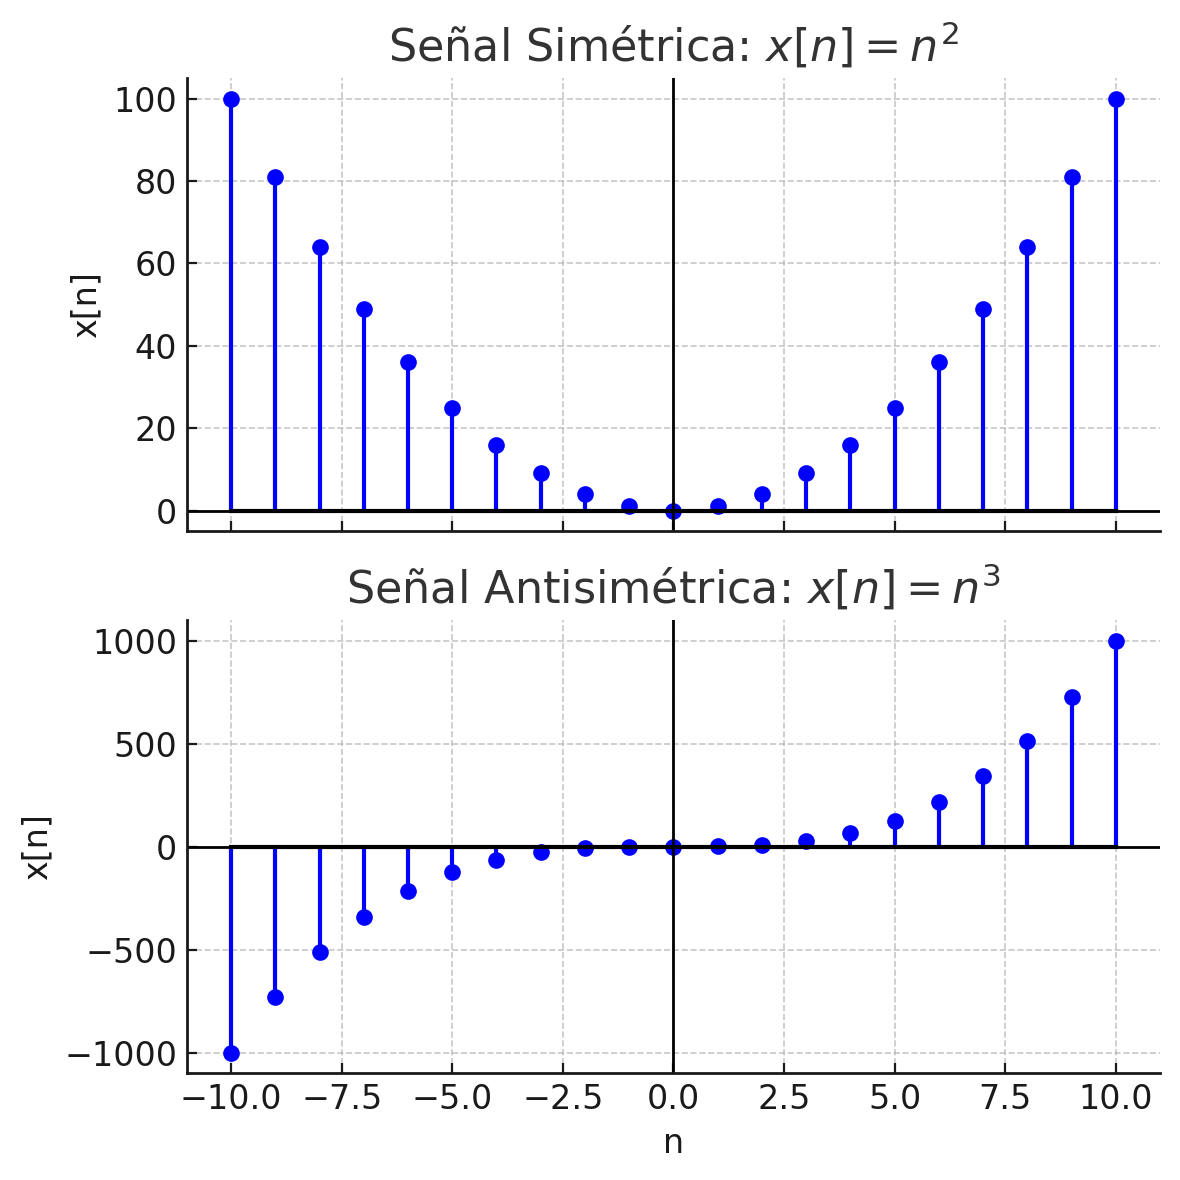
\includegraphics[width=0.5\textwidth]{Auxiliar_2_2.png}
      \caption{Ejemplos de señales simétricas y anti-simétricas.}
    \end{figure}
  \end{column}
  \begin{column}{0.45\textwidth}
    \begin{block}{Señales simétricas y anti-simétricas}
      \small
      \begin{itemize}
        \item Una señal \(x[n]\) es \textbf{simétrica} si \(x[n] = x[-n]\).
        \item Una señal \(x[n]\) es \textbf{anti-simétrica} si \(x[n] = -x[-n]\).
      \end{itemize}
    \end{block}
    \begin{figure}
      \centering
      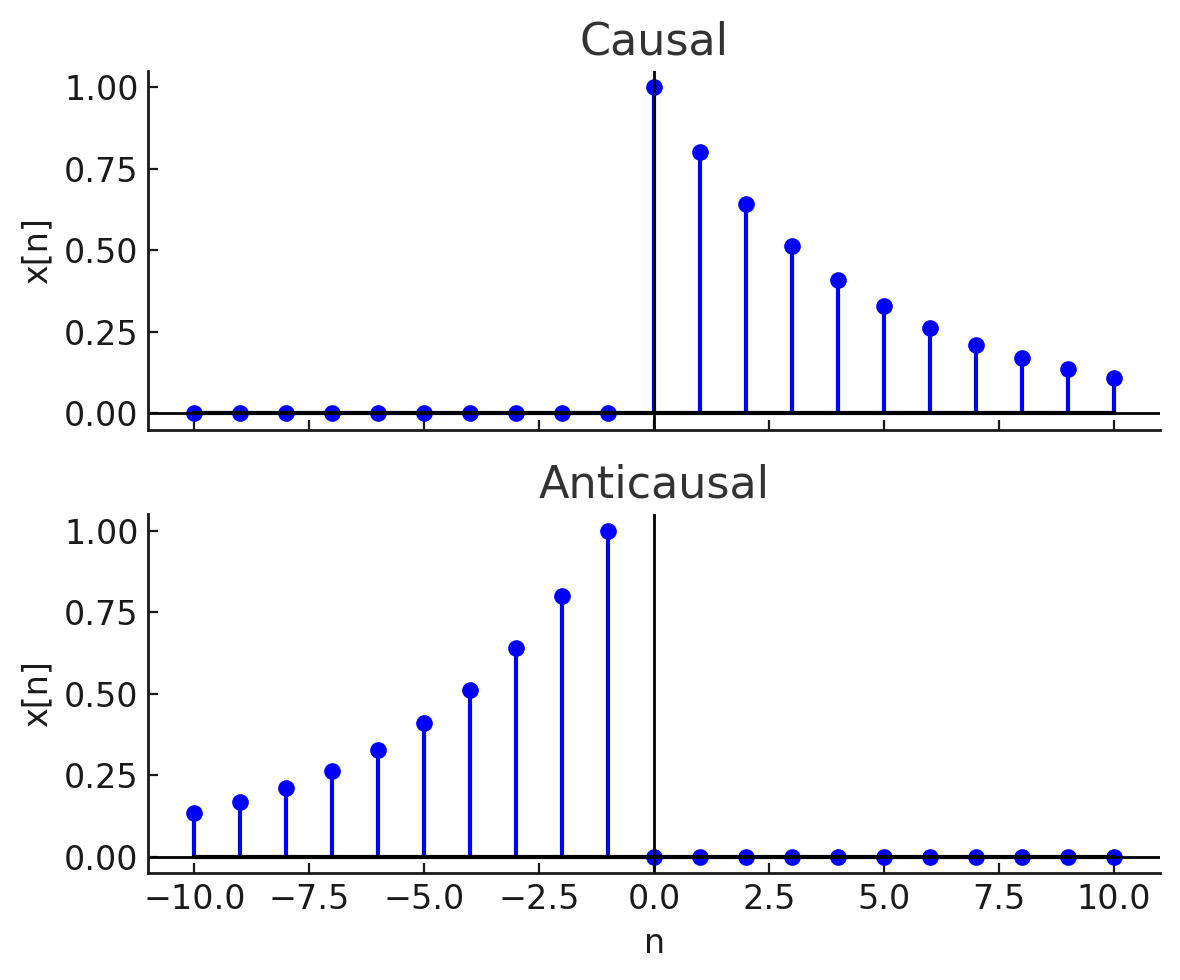
\includegraphics[width=0.5\textwidth]{Auxiliar_2_1.png}
      \caption{Ejemplos de señales causales y anticausales.}
    \end{figure}
  \end{column}
\end{columns}

\end{frame}
%---------------------
\begin{frame}{Simetría en señales discretas: pares e impares}
\begin{columns}[T,onlytextwidth]
  \begin{column}{0.55\textwidth}
    \begin{block}{Propiedad}
    Toda señal $x[n]_{n \in \mathbb{Z}}$ tiene una parte \textbf{simétrica} y una parte \textbf{anti-simétrica}:
    \begin{align*}
      x[n] &= x_s[n] + x_a[n], \\
      x_s[n] &= \tfrac{1}{2}\big(x[n] + x[-n]\big), \\
      x_a[n] &= \tfrac{1}{2}\big(x[n] - x[-n]\big).
    \end{align*}
    \end{block}
  \end{column}
  \begin{column}{0.4\textwidth}
    \begin{figure}
      \centering
      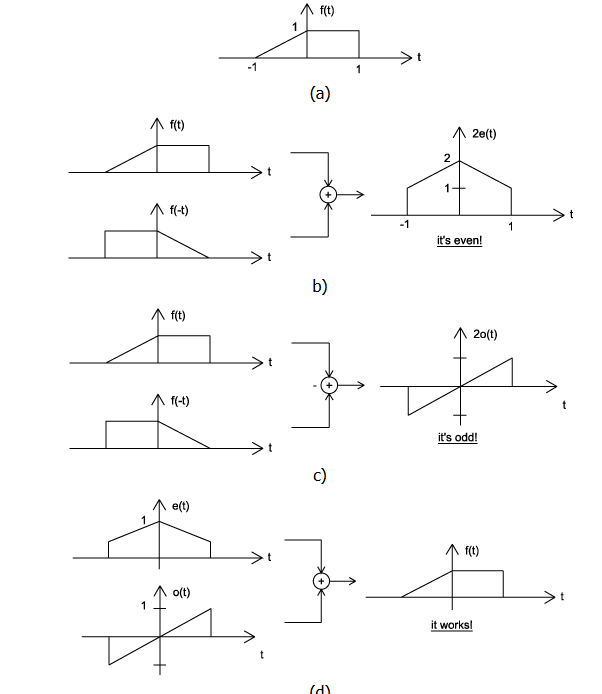
\includegraphics[width=0.9\linewidth]{Auxiliar_2_3.png}
      \caption{\scriptsize Ejemplo de descomposición par/impar.}
    \end{figure}
  \end{column}
\end{columns}
\end{frame}
%---------------------
\begin{frame}{Funciones clásicas en tiempo discreto}
\begin{columns}[T,onlytextwidth]
  \begin{column}{0.55\textwidth}
  \begin{block}{Funciones clásicas}
      \small
    \begin{itemize}
  \item \textbf{Impulso}
  \begin{equation}
    \delta[n]=
    \begin{cases}
      1, & n=0,\\
      0, & n\neq 0.
    \end{cases}
  \end{equation}

  \item \textbf{Escalón}
  \begin{equation}
    u[n]=
    \begin{cases}
      1, & n\ge 0,\\
      0, & n<0.
    \end{cases}
  \end{equation}

  \item \textbf{Rampa}
  \begin{equation}
    r[n]=
    \begin{cases}
      n, & n\ge 0,\\
      0, & n<0.
    \end{cases}
  \end{equation}

  \item \textbf{Exponencial compleja}
  \begin{align}
    x[n] &= A\,(re^{j\theta})^{n},\\
    x[n] &= A\,r^{n}e^{j\theta n}.
  \end{align}
\end{itemize}
    \end{block}
  \end{column}
  \begin{column}{0.4\textwidth}
    \begin{figure}
      \centering
      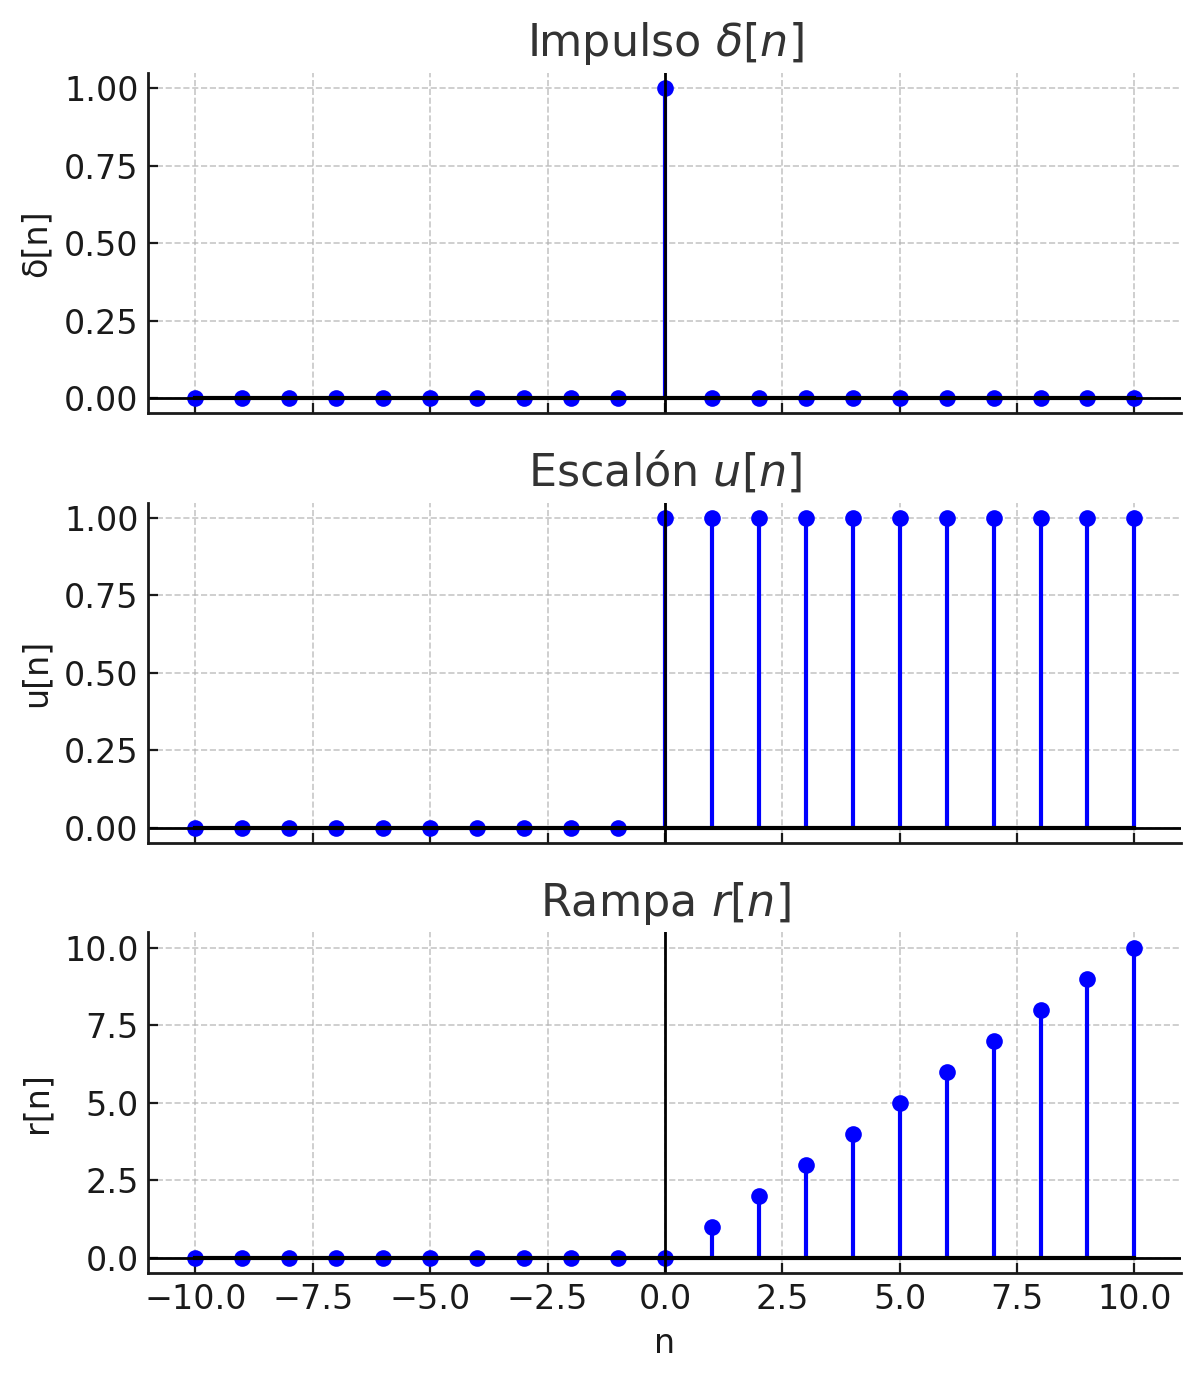
\includegraphics[width=0.9\linewidth]{Auxiliar_2_4.png}
  \caption{\scriptsize Ejemplo de funciones clásicas.}
    \end{figure}
  \end{column}
\end{columns}
\end{frame}

%----------------------------
\begin{frame}{Sistemas LTI}
    \begin{block}{Definición (discreto)}
      \footnotesize
      Un sistema $T$ es \textbf{lineal e invariante en el tiempo (LTI)} si cumple:
      \begin{itemize}
        \item \textbf{Linealidad (principio de superposición):}\\
        Para cualesquiera señales $x_1[n], x_2[n]$ y escalares $\alpha, \beta \in \mathbb{R}$,
        \begin{equation*}
          T\{\alpha x_1[n] + \beta x_2[n]\} = \alpha T\{x_1[n]\} + \beta T\{x_2[n]\}.
        \end{equation*}

        \item \textbf{Invariancia en el tiempo:}\\
        El comportamiento del sistema no cambia si la entrada se desplaza en el tiempo. Es decir, para todo $k \in \mathbb{Z}$,
        \begin{equation*}
          T\{x[n-k]\} = y[n-k], \quad \text{donde } y[n] = T\{x[n]\}.
        \end{equation*}

        \item \textbf{Respuesta al impulso y convolución:}\\
        La dinámica del sistema queda completamente caracterizada por su \textbf{respuesta al impulso}
        \begin{equation*}
          h[n] = T\{\delta[n]\}.
        \end{equation*}
        La salida para cualquier entrada $x[n]$ se obtiene mediante la \textbf{convolución}:
        \begin{equation*}
          y[n] = (x * h)[n] = \sum_{k \in \mathbb{Z}} x[k]\, h[n-k].
        \end{equation*}
      \end{itemize}
    \end{block}
\end{frame}


%----------------------------
\section{Pregunta 1}
\begin{frame}{Pregunta \#1}
\begin{block}{Enunciado Pregunta \#1}
 Sean los siguientes sistemas a tiempo discreto:

\begin{enumerate}
\item Determine si los siguientes sistemas a tiempo discreto son lineales y/o invariantes en el tiempo:
\begin{itemize}
\item $y[n] = nx[n]$
\item $y[n] = e^{x[n]}$
\item $y[n] = \sum_{j=1}^{M} a_j \cdot x[n-j] + B$
\end{itemize}

\item Para el sistema a tiempo discreto T definido por la relación entrada-salida $y[n] = nx[n]$ bosqueje por separado $T_2(T((x[n])))$ y $T(T_2((x[n])))$ y compare con los resultados obtenidos en la parte a. Para el bosquejo considere la señal:
\begin{equation}
x[n] = \begin{cases}
1 & 0 \leq n \leq 2 \\
0 & \text{en otro caso}
\end{cases}
\end{equation}
\end{enumerate}
\end{block}
\end{frame}
%-----------------------------
\begin{frame}{Señal de prueba $x[n]$}
\begin{figure}
  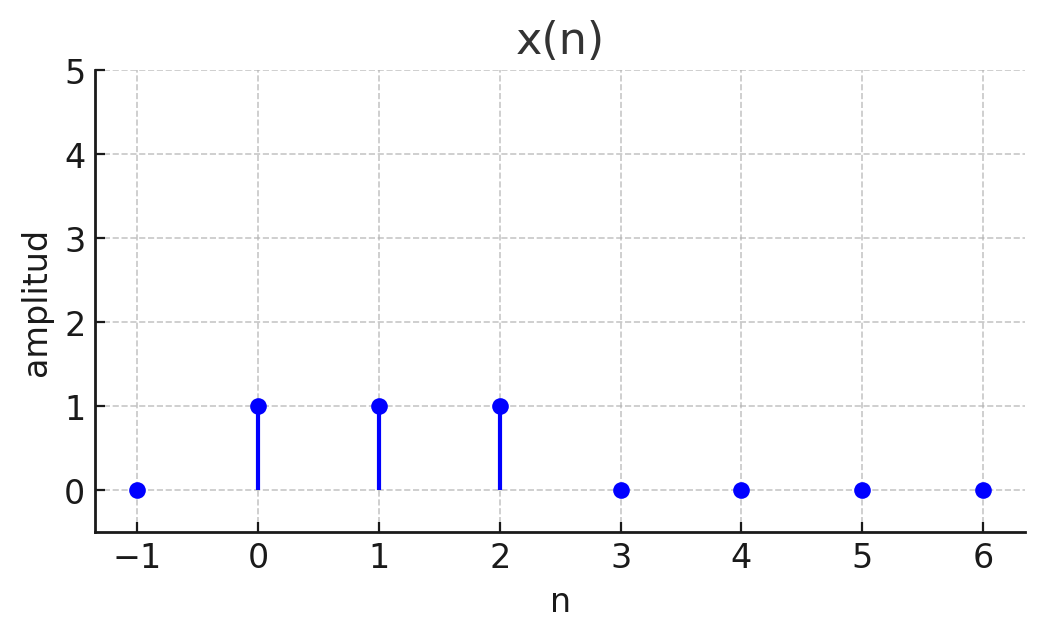
\includegraphics[width=0.7\textwidth]{../figures/Auxiliar_2_1.png}
  \caption{\scriptsize Señal discreta $x[n]$.}
\end{figure}
\end{frame}
%-----------------------------
\begin{frame}{Comparación de $T_2\circ T$ vs. $T\circ T_2$}
\begin{figure}
  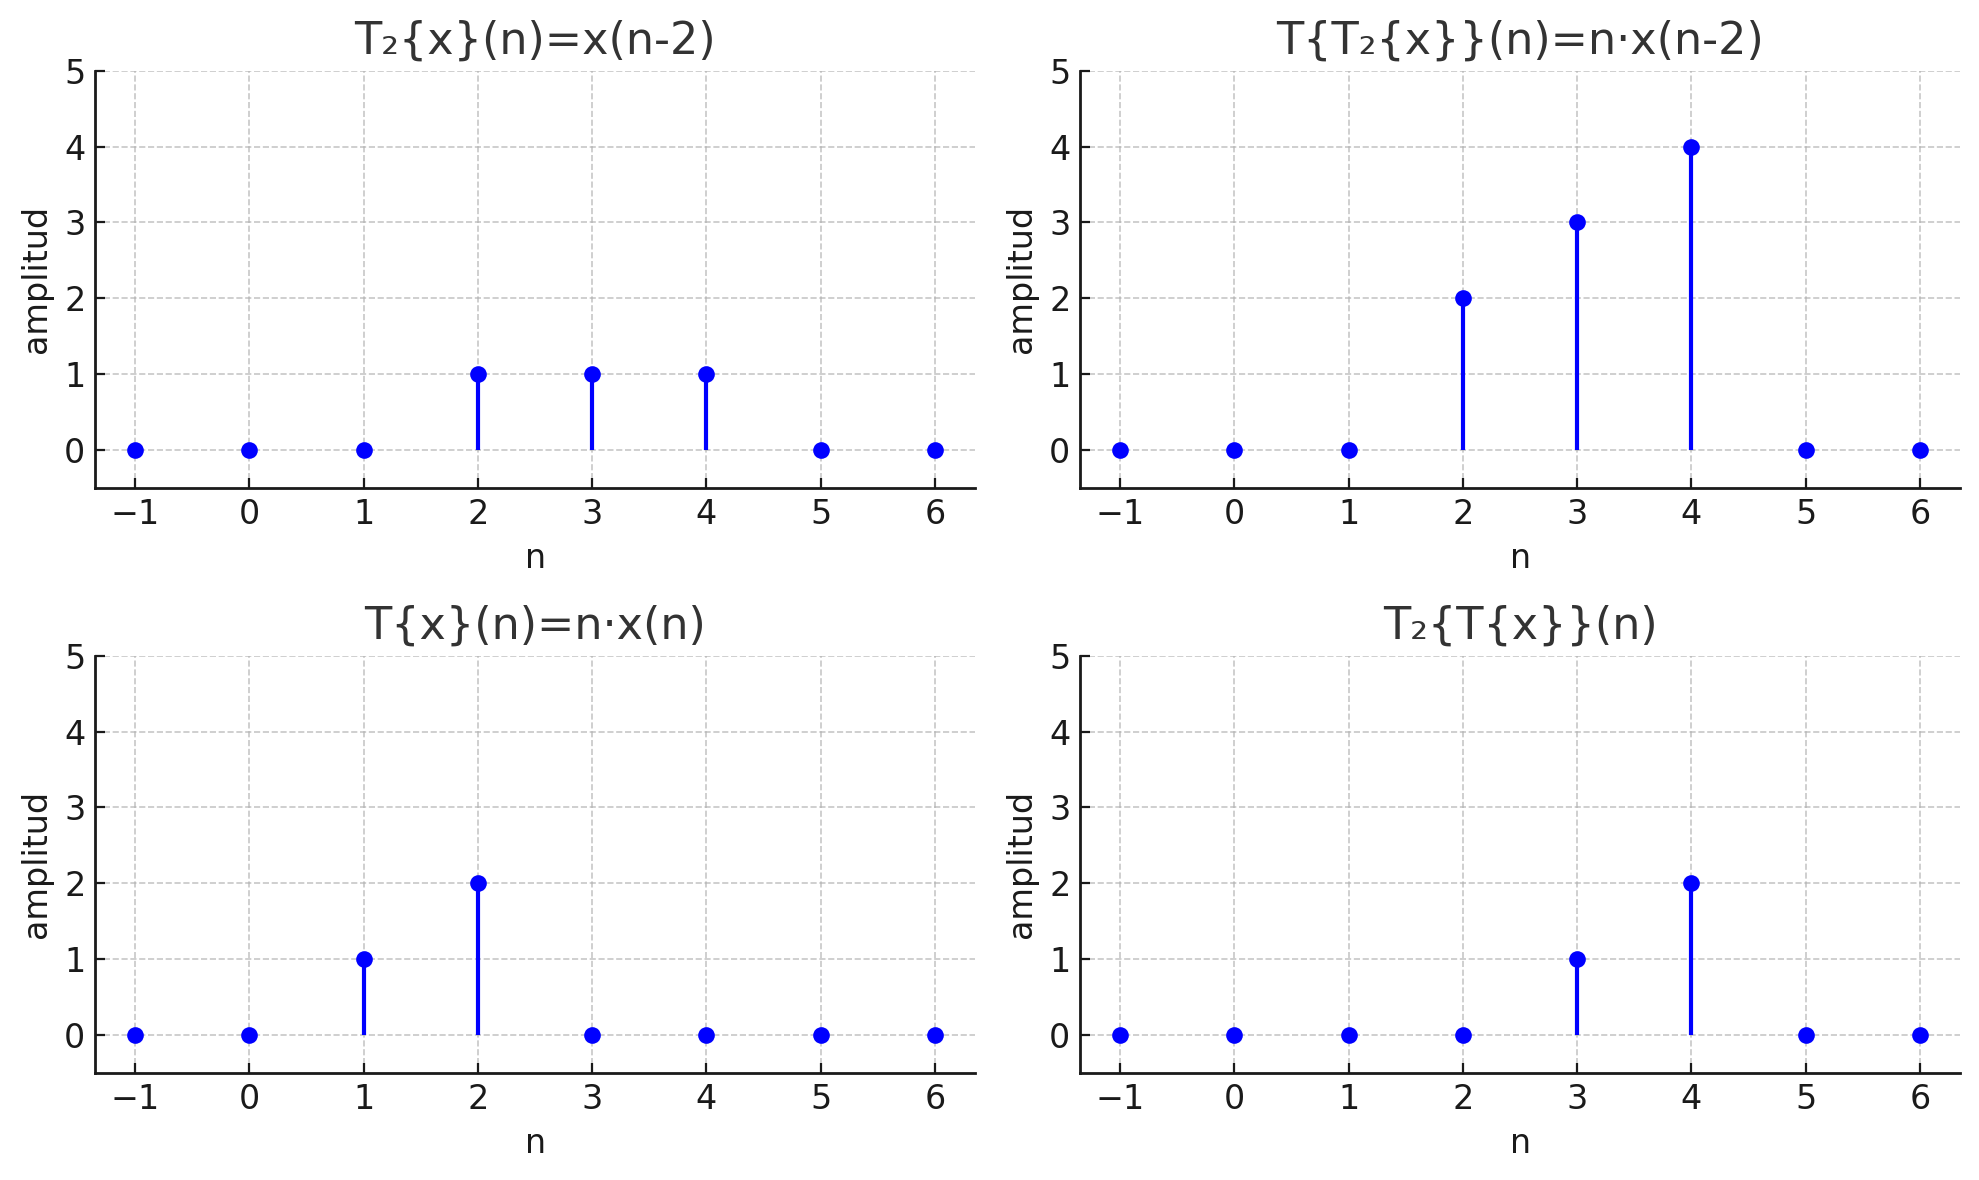
\includegraphics[width=0.8\textwidth]{../figures/Auxiliar_2_2.png}
  \caption{\scriptsize Arriba izq.: $T_2\{x\}(n)=x(n-2)$. Arriba der.: $T\{T_2\{x\}\}(n)=n\,x(n-2)$. Abajo izq.: $T\{x\}(n)=n\,x(n)$. Abajo der.: $T_2\{T\{x\}\}(n)=(n-2)\,x(n-2)$. Se verifica que $T_2\circ T\ne T\circ T_2$; por lo tanto, $T$ no es invariante en el tiempo.}
\end{figure}
\end{frame}
%-----------------------------
\section{Pregunta 2}
\begin{frame}{Pregunta \#2}
\begin{block}{Enunciado Pregunta \#2}
 Escriba el siguiente sistema, bosqueje la salida del sistema si a la entrada hay un impulso de magnitud 1 centrado en 0 y clasifique esa señal de salida en cuanto a su energía y si corresponde, su potencia.
\end{block}
\begin{figure}[H]
  \centering
  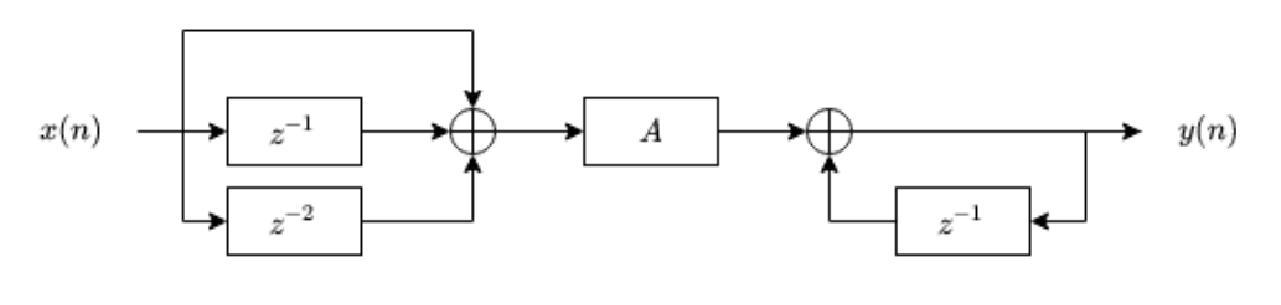
\includegraphics[width=0.8\textwidth]{Auxiliar_2_5}
\end{figure}
\end{frame}
%%%%%%%%%%%%%%%%%%%%%%
\begin{frame}
\begin{figure}
  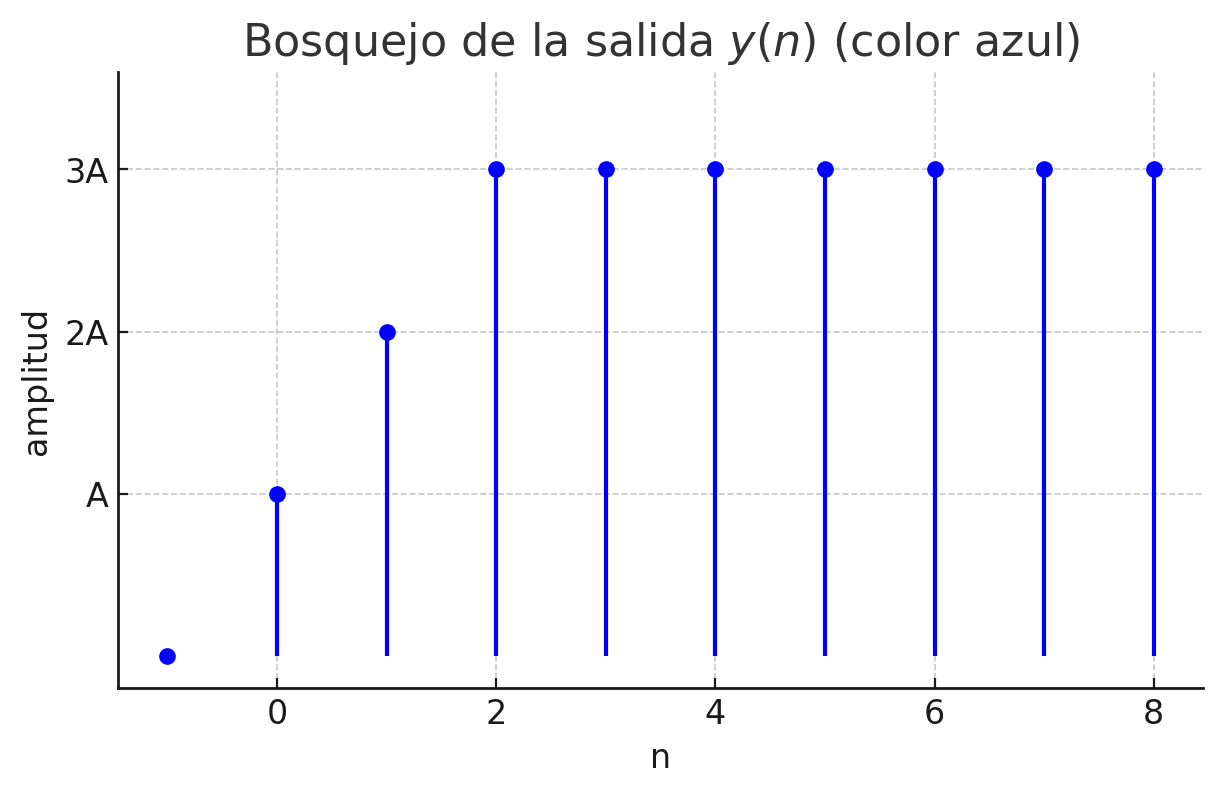
\includegraphics[width=0.52\textwidth]{Auxiliar_2_6}
  \caption{Señal de salida del sistema para un impulso de magnitud 1 centrado en 0}
\end{figure}
\end{frame}
%%%%%%%%%%%%%%%%%%%%%%
\section{Pregunta 3}
\begin{frame}{Pregunta \#3}
\begin{block}{Enunciado Pregunta \#3}
Considere el sistema mostrado en la figura, donde \(h[n]=a^n u[n]\) con \(-1<a<1\). Determine la respuesta del sistema bajo la excitación
\[x[n]=u[n+5]-u[n-10].\]
\end{block}
\begin{figure}[H]
  \centering
  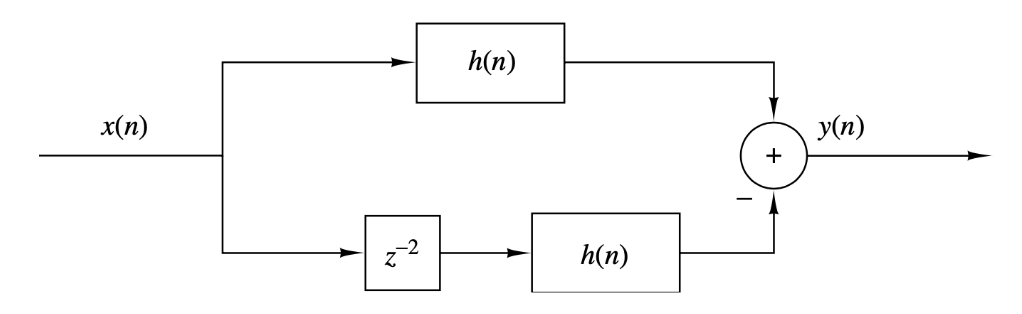
\includegraphics[width=0.7\textwidth]{Auxiliar_2_7}
  \caption{Sistema a analizar.}
\end{figure}
\end{frame}
%-------------------------------
\section{Pregunta 4}
\begin{frame}{Pregunta \#4}
\begin{block}{Enunciado Pregunta \#4}
Demuestre que, si un sistema cumple
\[ y[n]=T\{x[n]\}=x[n]*h[n]=\sum_{k\in\mathbb{Z}} x[k] \, h[n-k], \]
entonces, con \(h[n]\) la respuesta al impulso del sistema, necesariamente el sistema es lineal e invariante en el tiempo (LTI).
\end{block}
\end{frame}
%---------------------------
\section{Pregunta 5}
\begin{frame}{Pregunta \#5}
\begin{block}{Enunciado Pregunta \#5}
  Tres sistemas con respuestas al impulso \(h_1[n]=\delta[n]-\delta[n-1]\), \(h_2[n]=h[n]\) y \(h_3[n]=u[n]\) se conectan en cascada.
\begin{enumerate}
  \item ¿Cuál es la respuesta al impulso total \(h_c[n]\) del sistema en su conjunto?
  \item ¿El orden de conexión afecta al sistema en su conjunto? Justifique.
\end{enumerate}
\end{block}
\end{frame}
%---------------------------
\section{Pregunta 6}
\begin{frame}{Pregunta \#6}
\begin{block}{Enunciado Pregunta \#6}
  Considere el sistema a tiempo discreto de orden $N$ caracterizado por la siguiente ecuación de diferencia de parámetros $b_1,\ldots,b_N$ y $a_0,\ldots,a_M$:
\begin{equation}
\label{eq:edo}
 y(n) = b_1 y(n-1)+\cdots+b_N y(n-N) + a_0 x(n)+\cdots+a_M x(n-M),
\end{equation}
para todo $n\in\mathbb{Z}$.

\begin{enumerate}
  \item Verifique que el sistema determinado en la Ec es lineal.
  \item Verifique que el sistema determinado en la Ec es invariante en el tiempo (TI).
\end{enumerate}
\end{block}
\end{frame}

\begin{frame}
  \begin{block}{Continuacion Enunciado \#6}
    \begin{enumerate}
      \item Considere la versión con condiciones iniciales del sistema en \eqref{eq:edo}, es decir, $y(n)$ se determina para $n\ge 0$ donde la entrada es $\big(x(n)\big)_{n\ge 0}$ (asumiendo valores nulos en tiempos negativos) y el vector de estado (condiciones iniciales de \eqref{eq:edo}) es $y_1=y(-1),\ldots,y_N=y(-N)$. Verifique que la solución frente a la entrada $\big(x(n)\big)_{n\ge 0}$ y las condiciones iniciales $(y_1,\ldots,y_N)$ se puede escribir como
  \begin{equation}
    \big(y(n)\big)_{n\ge 0} = \big(y_{SO}(n)\big)_{n\ge 0} + \big(y_{IO}(n)\big)_{n\ge 0},
  \end{equation}
  donde $\big(y_{SO}(n)\big)_{n\ge 0}$ denota la \emph{respuesta de estado cero} y $\big(y_{IO}(n)\big)_{n\ge 0}$ denota la \emph{respuesta de entrada cero}.
  \item Bajo el setting del punto (c), verifique que la relación $\big(x(n)\big)_{n\ge 0} \mapsto \big(y_{SO}(n)\big)_{n\ge 0}$ determina un sistema LTI.
  \item Bajo el setting del punto (c), verifique que la relación $(y_1,\ldots,y_N) \mapsto \big(y_{IO}(n)\big)_{n\ge 0}$ es lineal.
\end{enumerate}
  \end{block}
\end{frame}
\end{document}
%--------------------------------
